\section{Results}\label{sec:results}

Unless stated otherwise, ``NAE'' refers to record-sampled queries with $k\ge2$ predicates, which is the
workload definition of~\cite{omni}; single-predicate queries are reported separately because a plain
Count-Min counter already answers them well.

\subsection{Accuracy at equal memory}\label{sec:acc}

\begin{figure}[t]
\centering
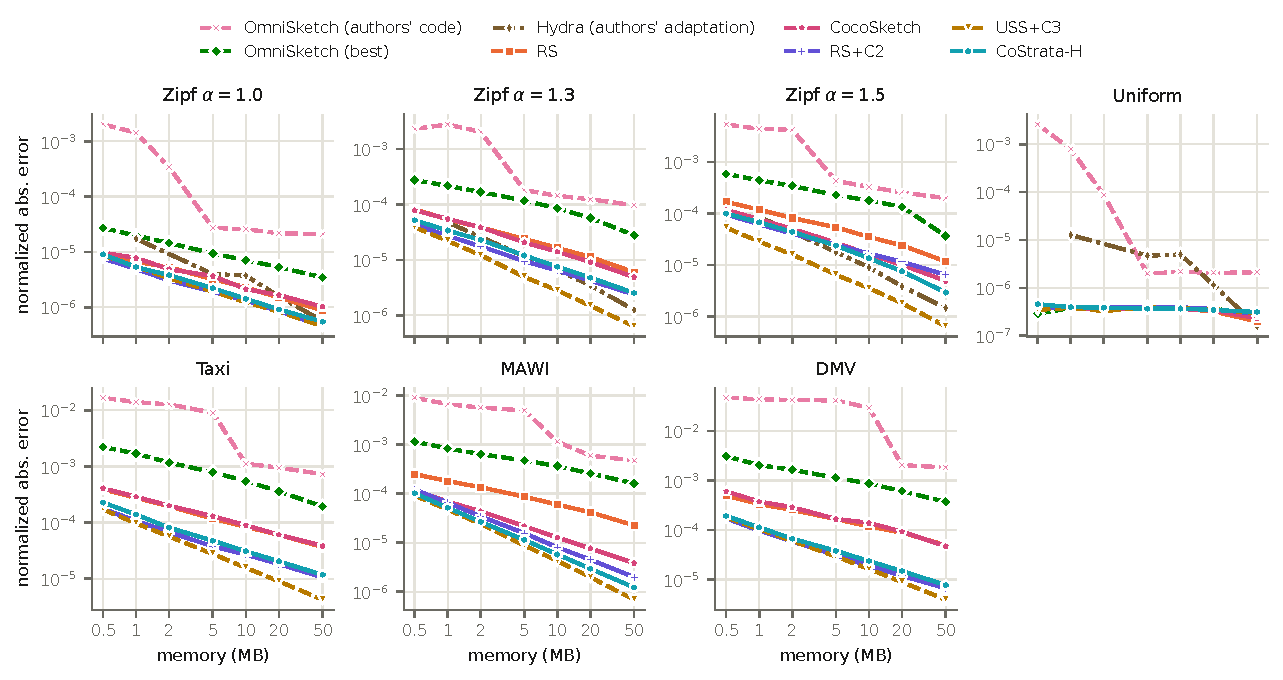
\includegraphics[width=\textwidth]{figs/nae_vs_mem.pdf}
\caption{Normalized absolute error on record-sampled queries with $k\ge2$ predicates versus memory
(mean of 5 seeds; lower is better). ``\omni (best cfg.)'' is the best of eight configurations under
oracle memory accounting, chosen separately for every point.}
\label{fig:nae}
\end{figure}

\begin{table}[t]
\centering\small
\caption{Normalized absolute error, record-sampled queries with $k\ge2$ predicates (mean of 5 seeds).
Bold: best method per column and budget.}
\label{tab:main}
\begin{tabular}{lrrrrrr}
\toprule
Method & Zipf $\alpha{=}1.0$ & Zipf $\alpha{=}1.3$ & Zipf $\alpha{=}1.5$ & Uniform & Taxi & MAWI \\
\midrule
\multicolumn{7}{l}{\emph{1 MB}} \\
OmniSketch {\footnotesize(paper)} & 3.4e-5 & 3.7e-4 & 8.1e-4 & 1.7e-6 & 2.7e-3 & 1.5e-3 \\
OmniSketch {\footnotesize(best cfg.)} & 2.1e-5 & 2.2e-4 & 4.4e-4 & \textbf{3.8e-7} & 1.8e-3 & 8.3e-4 \\
Reservoir {\footnotesize(RS)} & \textbf{6.7e-6} & 5.4e-5 & 1.2e-4 & 4.0e-7 & 2.7e-4 & 1.8e-4 \\
USS & 8.2e-6 & 5.9e-5 & 7.9e-5 & 4.2e-7 & 3.1e-4 & 6.0e-5 \\
RS+C & 7.7e-6 & 6.2e-5 & 1.3e-4 & 4.1e-7 & 2.2e-4 & 1.1e-4 \\
USS+C & 7.6e-6 & \textbf{5.3e-5} & \textbf{7.7e-5} & 4.2e-7 & \textbf{2.1e-4} & \textbf{5.9e-5} \\
CoStrata & 8.0e-6 & 7.5e-5 & 1.7e-4 & 4.1e-7 & 2.6e-4 & 1.2e-4 \\
\midrule
\multicolumn{7}{l}{\emph{10 MB}} \\
OmniSketch {\footnotesize(paper)} & 2.0e-5 & 1.6e-4 & 3.1e-4 & 1.4e-6 & 1.4e-3 & 6.0e-4 \\
OmniSketch {\footnotesize(best cfg.)} & 8.4e-6 & 1.0e-4 & 1.8e-4 & 3.8e-7 & 5.6e-4 & 3.8e-4 \\
Reservoir {\footnotesize(RS)} & \textbf{2.3e-6} & 1.6e-5 & 3.5e-5 & \textbf{3.7e-7} & 8.4e-5 & 5.9e-5 \\
USS & 2.5e-6 & 1.5e-5 & \textbf{1.7e-5} & 3.8e-7 & 9.4e-5 & 1.1e-5 \\
RS+C & 2.8e-6 & 1.9e-5 & 3.9e-5 & 3.9e-7 & 7.4e-5 & 2.7e-5 \\
USS+C & 2.6e-6 & \textbf{1.4e-5} & 1.8e-5 & 3.8e-7 & \textbf{6.5e-5} & \textbf{1.0e-5} \\
CoStrata & 2.9e-6 & 2.3e-5 & 5.0e-5 & 3.9e-7 & 8.2e-5 & 2.8e-5 \\
\bottomrule
\end{tabular}

\end{table}

\paragraph{Sanity check of the \omni re-implementation.} For three-predicate queries at 10\,MB---the
setting of Fig.~6 of~\cite{omni}---our implementation with the paper's parameters yields an NAE of
\NumOmniPaperKthreeZipfTen, \NumOmniPaperKthreeZipfThirteen{} and \NumOmniPaperKthreeZipfFifteen{} on the
Zipf streams with $\alpha=1.0, 1.3, 1.5$ and \NumOmniPaperKthreeUnif{} on the uniform stream. The
original figure shows the same qualitative picture (an error close to zero for the uniform stream that
grows with $\alpha$ to a few $10^{-4}$); an exact match cannot be expected because hash functions and
query samples differ.

\paragraph{Row sampling versus \omni.} Figure~\ref{fig:nae} and Table~\ref{tab:main} show the main
result. Across all six streams and seven budgets, the row reservoir has a
\NumOmniPaperVsResLo--\NumOmniPaperVsResHi$\times$ lower error than \omni with the published
parameters (geometric mean \NumOmniPaperVsResGm$\times$). Tuning does not close the gap: on the five
non-uniform streams, the best of the eight \omni configurations under oracle accounting is still
\NumOmniBestVsResLo--\NumOmniBestVsResHi$\times$ worse than the reservoir (geometric mean
\NumOmniBestVsResGm$\times$). The only tie is the Uniform stream, where multi-predicate queries match one or
two records, every method essentially returns zero, and the ratio is
\NumOmniBestVsResUnifLo--\NumOmniBestVsResUnifHi. Including single-predicate queries makes the published
configuration look worse (\NumOmniPaperVsResAllLo--\NumOmniPaperVsResAllHi$\times$, geometric mean
\NumOmniPaperVsResAllGm$\times$), because with $w=8$ columns it is a very coarse Count-Min sketch.
The shape of the curves confirms the analysis of Section~\ref{sec:anatomy}: the error of every
sample-based synopsis falls roughly as $M^{-1/2}$, whereas that of \omni (paper) flattens---on the
Uniform stream it stays between $\NumOmniPaperFlatLo\cdot10^{-6}$ and $\NumOmniPaperFlatHi\cdot10^{-6}$
over a hundred-fold increase in memory---because the collision term of
Proposition~\ref{prop:bias} does not depend on $B$. No single configuration wins the search: the published $(w,d)=(8,3)$ with lean accounting or $(64,2)$ is best
at small and medium budgets, and $(4096,1)$ at the largest ones, i.e., large budgets are better spent on
width than on ever larger per-cell samples.

\begin{table}[t]
\centering\footnotesize\setlength{\tabcolsep}{3.5pt}
\caption{NAE by number of predicates $k$ at 10\,MB, record-sampled queries (mean of 5 seeds).}
\label{tab:byk}
\begin{tabular}{lrrrrrrrrrrrr}
\toprule
 & \multicolumn{6}{c}{Taxi, number of predicates $k$} & \multicolumn{6}{c}{MAWI, number of predicates $k$} \\
Method & 1 & 2 & 3 & 4 & 5 & 6 & 1 & 2 & 3 & 4 & 5 & 6 \\
\midrule
Omni. (paper) & 3.2e-3 & 4.1e-3 & 2.1e-3 & 7.3e-4 & 1.6e-4 & 6.9e-5 & 2.3e-3 & 1.4e-3 & 7.5e-4 & 3.3e-4 & 2.6e-4 & 2.6e-4 \\
Omni. (best cfg.) & 1.7e-5 & 1.3e-3 & 9.5e-4 & 4.0e-4 & 9.4e-5 & 4.7e-5 & 8.7e-5 & 7.6e-4 & 4.5e-4 & 1.6e-4 & 1.4e-4 & 1.4e-4 \\
RS & 2.7e-4 & 2.1e-4 & 1.3e-4 & \textbf{5.0e-5} & \textbf{1.6e-5} & \textbf{8.3e-6} & 1.4e-4 & 1.1e-4 & 7.9e-5 & 3.9e-5 & 3.3e-5 & 3.1e-5 \\
USS & 3.0e-4 & 2.3e-4 & 1.5e-4 & 6.1e-5 & 1.8e-5 & 8.9e-6 & 5.4e-5 & 2.8e-5 & 1.9e-5 & \textbf{4.4e-6} & \textbf{3.5e-6} & \textbf{1.6e-6} \\
RS+C & 3.9e-6 & 1.6e-4 & 1.2e-4 & 5.8e-5 & 1.8e-5 & 1.0e-5 & 6.8e-6 & 5.3e-5 & 3.7e-5 & 1.7e-5 & 1.5e-5 & 1.1e-5 \\
USS+C & \textbf{1.8e-6} & \textbf{1.4e-4} & \textbf{1.1e-4} & 5.1e-5 & 1.7e-5 & 8.4e-6 & \textbf{2.9e-6} & \textbf{2.3e-5} & \textbf{1.5e-5} & 5.5e-6 & 4.9e-6 & 3.6e-6 \\
CoStrata & 4.3e-6 & 1.8e-4 & 1.4e-4 & 6.3e-5 & 2.0e-5 & 1.1e-5 & 7.1e-6 & 5.4e-5 & 4.0e-5 & 1.9e-5 & 1.6e-5 & 1.3e-5 \\
\bottomrule
\end{tabular}

\end{table}

\paragraph{Calibration.} Table~\ref{tab:byk} breaks the error down by the number of predicates. For
$k=1$ the calibrated synopses (\textsc{RS+C}, \textsc{USS+C}, \cs) are one to two orders of magnitude more
accurate than the uncalibrated samples, simply because the estimate is tied to an exact counter of a
fine-grained bucket. This is where most of the overall gain of calibration comes from: over all $k$,
\textsc{RS+C} improves on RS by a geometric mean of \NumCalibRsAllGm$\times$
(\NumCalibRsAllLo--\NumCalibRsAllHi$\times$) and \textsc{USS+C} on USS by \NumCalibUssAllGm$\times$. For
$k\ge2$ the picture is mixed and data dependent: calibration helps on MAWI
(\NumCalibRsMawiLo--\NumCalibRsMawiHi$\times$), where attributes are strongly correlated and a query
often covers most of its lightest bucket, helps slightly on Taxi
(\NumCalibRsTaxiLo--\NumCalibRsTaxiHi$\times$), and \emph{hurts} on the synthetic streams with independent
attributes (\NumCalibRsSynLo--\NumCalibRsSynHi$\times$, geometric mean \NumCalibRsSynGm$\times$), where the
marginal count carries little information about a conjunction and the calibrated sample simply holds fewer
rows (it pays for the counters, a 64-bit priority per row, and compaction slack). Over all streams the
geometric-mean gain for $k\ge2$ is \NumCalibRsGm$\times$.

\paragraph{USS.} Where full tuples repeat, aggregating them pays off: on MAWI (25\% distinct tuples) USS is
\NumUssVsResMawiLo--\NumUssVsResMawiHi$\times$ more accurate than the reservoir and, with calibration,
the most accurate method overall; the same holds, to a lesser degree, for the Zipf stream with
$\alpha=1.5$ (49\% distinct tuples). On Taxi (97\% distinct tuples) USS is slightly worse than the reservoir
because of its per-entry overhead. Across the board, \textsc{USS+C} is the best or close to the best
method in Table~\ref{tab:main}.

\paragraph{\cs on frequent queries.} On this workload, which is dominated by frequent values, \cs is
\NumCsVsRscLo--\NumCsVsRscHi$\times$ (geometric mean \NumCsVsRscGm$\times$) less accurate than the calibrated
uniform sample \textsc{RS+C}: this is the price of reserving half of the nominal budget for the hash
strata, and it stays well within the $\sqrt2$ bound of Proposition~\ref{prop:size}. Relative to the plain
reservoir \cs ranges from $1/\NumCsVsResLo\approx2\times$ better (MAWI) to \NumCsVsResHi$\times$ worse
(Zipf streams), with a geometric mean of \NumCsVsResGm. \cs is therefore not a better
general-purpose estimator for frequent conjunctions; its purpose is the regime discussed next.

\subsection{Rare anchors: when stratification pays}\label{sec:anchor}

\begin{figure}[t]
\centering
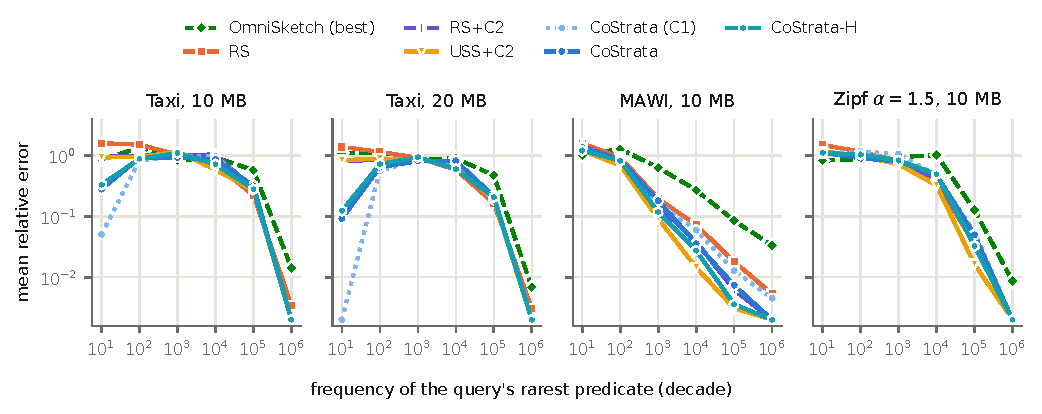
\includegraphics[width=\textwidth]{figs/anchor.pdf}
\caption{Mean relative error of anchored queries, grouped by the frequency decade of the rarest
predicate (mean of 5 seeds). Values near 1 mean that the synopsis has essentially no information about
the query.}
\label{fig:anchor}
\end{figure}

Figure~\ref{fig:anchor} groups anchored queries by the frequency of their rarest predicate.
On Taxi, whose attributes have between 4 and 697 distinct values, most values own a bucket, and \cs
guarantees each of them about $B$ sampled rows. For anchors that occur 10--99 times, the mean relative
error of \cs is \NumTaxiDOneCsFive{} at 5\,MB, \NumTaxiDOneCsTen{} at 10\,MB and \NumTaxiDOneCsTwenty{} at
20\,MB, while the best competitor stays at \NumTaxiDOneOtherFive, \NumTaxiDOneOtherTen{} and
\NumTaxiDOneOtherTwenty, respectively---an improvement of \NumTaxiDOneGainFive$\times$,
\NumTaxiDOneGainTen$\times$ and more than two orders of magnitude; at 50\,MB all such queries are answered
essentially exactly, as predicted by Proposition~\ref{prop:rare} (the automatic $B$ exceeds the bucket
counts). For anchors occurring 100--999 times the gain is \NumTaxiDTwoGainTen$\times$ at 10\,MB and
\NumTaxiDTwoGainFifty$\times$ at 50\,MB. The effect needs a sufficient budget: at 1\,MB, $B\approx5$ and \cs
is indistinguishable from \textsc{RS+C}. For frequent anchors ($10^4$--$10^6$ occurrences) the relative error of \cs is
\NumTaxiFreqPenaltyLo--\NumTaxiFreqPenaltyHi$\times$ that of the reservoir, which again reflects its smaller
uniform share.

On MAWI and on the Zipf streams, stratification is neutral: the strata of IP addresses, ports, or of a
10\,000-value Zipf domain are all of comparable weight, and with tens of thousands of non-empty buckets
$B$ is between 2 and 30 rows, so the house stratum dominates. Here the ranking is determined by
calibration and, on MAWI, by tuple aggregation (USS and \textsc{USS+C} are best in every decade).
\omni does not benefit from its per-cell samples in either case: for rare anchors its relative error
is close to or above 1 for every configuration, because the usable rate is that of the heaviest cell
(Observation~\ref{obs:min}) and collisions inflate small counts.

\subsection{Update throughput and query latency}\label{sec:speed}

\begin{table}[t]
\centering\small
\caption{Update throughput and query latency on one core (median of 3 runs). Latency is the mean over the
2\,400 queries of the workload, after a one-time preparation pass (sorting cells for \omni, computing
weights for \cs).}
\label{tab:speed}
\begin{tabular}{lrrrrrr}
\toprule
 & \multicolumn{3}{c}{Taxi ($p{=}12$)} & \multicolumn{3}{c}{MAWI ($p{=}10$)} \\
Method & 1 MB & 10 MB & 50 MB & 1 MB & 10 MB & 50 MB \\
\midrule
\multicolumn{7}{l}{\emph{Update throughput (million records/s)}} \\
RS & 520.7 & -- & -- & -- & -- & -- \\
USS & 17.5 & -- & -- & -- & -- & -- \\
RS+C1 & 32.2 & -- & -- & -- & -- & -- \\
RS+C2 & 5.2 & -- & -- & -- & -- & -- \\
USS+C2 & 4.2 & -- & -- & -- & -- & -- \\
aSH & 3.2 & -- & -- & -- & -- & -- \\
OmniSketch (port of authors' code) & 13.7 & -- & -- & -- & -- & -- \\
OmniSketch (ours, same $B$) & 12.0 & -- & -- & -- & -- & -- \\
OmniSketch (journal cfg.) & 11.2 & -- & -- & -- & -- & -- \\
OmniSketch ($8{\times}3$, lean) & 10.5 & -- & -- & -- & -- & -- \\
OmniSketch ($256{\times}2$) & 14.2 & -- & -- & -- & -- & -- \\
OmniSketch ($1024{\times}2$) & 10.7 & -- & -- & -- & -- & -- \\
\midrule
\multicolumn{7}{l}{\emph{Query latency ($\mu$s per query)}} \\
RS & 22 & 229 & 1273 & 22 & 231 & 1274 \\
USS & 29 & 350 & 2821 & 28 & 328 & 2594 \\
OmniSketch (ours, same $B$) & 3.7 & 20 & 96 & 2.9 & 25 & 121 \\
OmniSketch ($256{\times}2$) & 1.0 & 9.5 & 68 & 0.6 & 4.5 & 22 \\
OmniSketch ($1024{\times}2$) & 0.6 & 7.1 & 52 & 0.2 & 1.3 & 5.5 \\
\bottomrule
\end{tabular}

\end{table}

Table~\ref{tab:speed} reports single-core performance. The reservoir is in a class of its own
(\NumTpResLo--\NumTpResHi{} million records/s) because skip counting touches only sampled records.
\cs ingests \NumTpCsLo--\NumTpCsHi{} million records/s: its per-record cost is $p$ hash evaluations and
counter increments, plus compactions, which become noticeable when the sample is a large fraction of the
stream (50\,MB is 11\% of Taxi). It is \NumTpCsVsOmniLo--\NumTpCsVsOmniHi$\times$ faster than the fastest
\omni configuration at every budget and at least as fast as USS, which must probe a hash table and update a
heap for every record. Our \omni re-implementation reaches
\NumTpOmniPaperLo--\NumTpOmniPaperHi{} million records/s with the published parameters; the original Java
implementation is reported at 0.09--0.2 million records/s on different hardware~\cite{omni}, so the
flat-heap and threshold-array engineering of Section~\ref{sec:setup} matters, and our accuracy
comparison is not against a slow strawman. With lean accounting the same budget buys four times
larger samples, and throughput drops to \NumTpOmniLeanLo{} million records/s at 50\,MB because heaps of
tens of thousands of entries are updated for a large part of the stream.

Query latency is the one dimension in which \omni is clearly ahead, at every budget: it merges $|Q|\,d$
sorted lists of at most $B$ hashes (\NumQlatOmniLo--\NumQlatOmniHi\,$\mu$s per query), whereas the row
samples scan the first predicate's column over the whole sample (\NumQlatCsLo--\NumQlatCsHi\,$\mu$s for \cs,
i.e., \NumQlatCsVsOmniPaperLo--\NumQlatCsVsOmniPaperHi$\times$ slower than \omni with the published parameters
and up to \NumQlatCsVsOmniHi$\times$ slower than its fastest configuration). \cs is somewhat faster than the
reservoir and USS because it holds fewer rows. For workloads with many queries per synopsis a per-bucket index on the row store would
make selective predicates sub-linear; we leave this to future work.

\subsection{Scaling the number of attributes}\label{sec:census}

\begin{figure}[t]
\centering
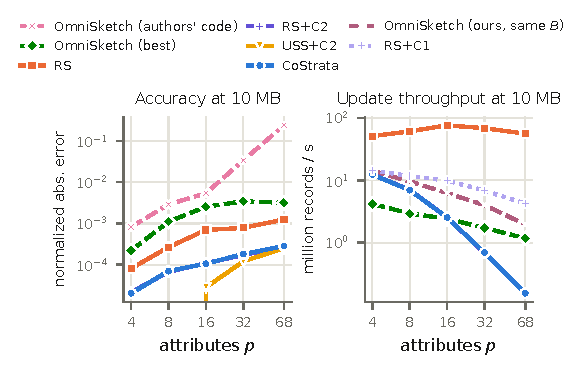
\includegraphics[width=\textwidth]{figs/census_scaling.pdf}
\caption{Census stream restricted to its first $p$ attributes, 10\,MB (accuracy: mean of 3 seeds;
throughput: one core, with $(w,d)=(256,2)$ for the ``best cfg.'' series).}
\label{fig:census}
\end{figure}

The main argument for \omni over Hydra is linear scaling in $p$. Row samples scale the same way---a row
costs $p$ words---and Figure~\ref{fig:census} shows that the accuracy ranking is unchanged from 4 to 68
attributes: at $p=68$ the reservoir is \NumCensusOmniBestVsResSixtyEight$\times$ more accurate than the
best \omni configuration, and \cs another \NumCensusResVsCsSixtyEight$\times$ more accurate than the
reservoir (Census attributes are correlated categorical variables, the favourable case for
calibration). For small $p$ the stream has few distinct tuples and USS is nearly exact; its advantage
shrinks as $p$ grows and has vanished at $p=68$. Throughput at $p=68$ is \NumCensusTpCsSixtyEight{} million
records/s for \cs and \NumCensusTpOmniSixtyEight{} for \omni (paper parameters).

\subsection{Ablations and estimator validity}\label{sec:ablation}

\begin{table}[t]
\centering\small
\caption{\cs design space at 10\,MB (mean of 5 seeds): NAE on record-sampled queries with $k\ge2$, and
mean relative error of anchored queries whose rarest predicate occurs 10--99 and 100--999 times.}
\label{tab:ablation}
\begin{tabular}{lrrrrrr}
\toprule
 & \multicolumn{3}{c}{Taxi} & \multicolumn{3}{c}{MAWI} \\
Variant & NAE & anchor $10^1$ & anchor $10^2$ & NAE & anchor $10^1$ & anchor $10^2$ \\
\midrule
\multicolumn{7}{l}{\emph{pair-table share} $\phi_2$ \emph{(uniform sample)}} \\
\quad none (RS+C1) & 7.2e-5 & 1.2 & 1.2 & 2.5e-5 & 1.4 & 0.84 \\
\quad $\phi_2=0.05$ & 2.9e-5 & 1.1 & 1.1 & 1.2e-5 & 1.4 & 0.85 \\
\quad $\phi_2=0.1$ & 2.7e-5 & 1.1 & 1.1 & 9.8e-6 & 1.4 & 0.89 \\
\quad $\phi_2=0.25$ (default) & 2.7e-5 & 0.94 & 1 & 8.0e-6 & 1.4 & 0.85 \\
\quad $\phi_2=0.5$ & 3.1e-5 & 0.94 & 0.8 & 7.1e-6 & 1.3 & 0.84 \\
\multicolumn{7}{l}{\emph{pair and triple tables} $\phi_2/\phi_3$} \\
\quad $0.1/0.1$ & 1.8e-5 & 1.1 & 1.1 & 9.6e-6 & 1.5 & 0.89 \\
\quad $0.15/0.15$ (RS+C3) & 1.7e-5 & 1 & 1.1 & 8.0e-6 & 1.4 & 0.88 \\
\quad $0.2/0.3$ & 1.5e-5 & 0.98 & 1 & 8.2e-6 & 1.4 & 0.96 \\
\multicolumn{7}{l}{\emph{all anchors (raking) instead of the lightest}} \\
\quad $\phi_2=0.25$, all anchors & 2.2e-5 & 1.1 & 1.2 & 1.1e-5 & 1.5 & 0.94 \\
\quad $0.15/0.15$, all anchors & 1.9e-5 & 1.4 & 1.3 & 1.8e-5 & 1.6 & 1 \\
\multicolumn{7}{l}{\emph{house weight} $\lambda$ \emph{(C1 only)}} \\
\quad $\lambda=0$ (strata only) & 1.9e-4 & 0.002 & 0.26 & 9.5e-5 & 1.2 & 0.83 \\
\quad $\lambda=1/4$ & 9.2e-5 & 0.0065 & 0.48 & 3.6e-5 & 1.3 & 0.86 \\
\quad $\lambda=1$ & 7.8e-5 & 0.051 & 0.83 & 2.6e-5 & 1.4 & 0.85 \\
\quad $\lambda=4$ & 7.3e-5 & 0.45 & 0.99 & 2.6e-5 & 1.4 & 0.85 \\
\multicolumn{7}{l}{\emph{house weight with pair tables}} \\
\quad $\lambda=1/4$, $\phi_2=0.25$ & 3.2e-5 & 0.12 & 0.68 & 1.0e-5 & 1.2 & 0.8 \\
\quad $\lambda=1$, $\phi_2=0.25$ (\cs) & 2.8e-5 & 0.28 & 0.92 & 8.5e-6 & 1.4 & 0.87 \\
\multicolumn{7}{l}{\emph{hold mode (}$\phi_2=0.25$\emph{)}} \\
\quad $\lambda=1/4$ & 3.8e-5 & 0.1 & 0.79 & 7.9e-6 & 1.2 & 0.8 \\
\quad $\lambda=1$ (\csh) & 3.1e-5 & 0.33 & 0.89 & 5.7e-6 & 1.2 & 0.82 \\
\quad $\lambda=4$ & 2.8e-5 & 0.59 & 0.79 & 5.0e-6 & 1.4 & 0.76 \\
\quad USS+C2 (no strata) & 2.6e-5 & 0.93 & 0.95 & 4.2e-6 & 1.2 & 0.69 \\
\multicolumn{7}{l}{\emph{allocation exponent} $\gamma$ \emph{(}$\lambda=0$\emph{, C1 only)}} \\
\quad $\gamma=0.75$ & 1.3e-4 & 0.0065 & 0.46 & 5.3e-5 & 1.2 & 0.81 \\
\quad $\gamma=0.5$ & 9.4e-5 & 0.32 & 0.81 & 3.5e-5 & 1.3 & 0.78 \\
\multicolumn{7}{l}{\emph{buckets per attribute} $w$ \emph{(}$\lambda=1$\emph{, C1 only)}} \\
\quad $w=64$ & 8.1e-5 & 0.83 & 1.1 & 4.7e-5 & 1.4 & 0.88 \\
\quad $w=256$ & 7.9e-5 & 0.4 & 0.84 & 4.0e-5 & 1.3 & 0.88 \\
\quad $w=1024$ & 7.8e-5 & 0.13 & 0.87 & 3.3e-5 & 1.3 & 0.86 \\
\quad $w=4096$ & 7.7e-5 & 0.052 & 0.81 & 2.8e-5 & 1.4 & 0.9 \\
\quad $w=16384$ & 8.1e-5 & 0.054 & 0.84 & 2.7e-5 & 1.3 & 0.86 \\
\multicolumn{7}{l}{\emph{reference}} \\
\quad RS & 8.4e-5 & 1.6 & 1.5 & 5.9e-5 & 1.6 & 0.94 \\
\bottomrule
\end{tabular}

\end{table}

\paragraph{House weight and allocation.} Table~\ref{tab:ablation} varies one design choice at a time.
The house weight $\lambda$ trades accuracy on frequent queries against accuracy on rare anchors exactly
as intended: without a house stratum ($\lambda=0$) rare anchors on Taxi are answered almost exactly but
the NAE is 2.5 times that of the reservoir; $\lambda=1$ gives up some of the rare-anchor gain and matches
the reservoir's NAE; $\lambda=1/4$ is a reasonable alternative when rare values matter most. A
sub-linear allocation exponent $\gamma<1$ without a house stratum is dominated by $\gamma=1$ with a
house stratum (compare $\gamma=0.5$ with $\lambda=1/4$: same NAE, 50 times larger error on rare anchors).
On MAWI none of these choices matters much for rare anchors, in line with Section~\ref{sec:anchor}.

\paragraph{Number of buckets.} On Taxi, rare-anchor accuracy improves until every value owns a bucket
($w\approx4096$) and is flat afterwards; on MAWI, larger $w$ improves the NAE because finer buckets make
calibration sharper. The automatic rule (5\% of the budget for counters) selects $w=8192$ at 10\,MB.

\paragraph{Calibrated versus Horvitz--Thompson estimates.} Over all record-sampled queries at 10\,MB, the
calibrated estimate of \cs has a \NumHtVsCalTaxi$\times$ (Taxi), \NumHtVsCalMawi$\times$ (MAWI) and
\NumHtVsCalZipf$\times$ (Zipf, $\alpha=1.5$) lower NAE than its HT estimate from the same sample.

\paragraph{Unbiasedness.} To check Theorem~\ref{thm:unbiased} empirically we ran \cs with many additional
independent seeds at budgets at which compactions are frequent: \NumBiasSeedsTaxi{} seeds on Taxi (1\,MB)
and \NumBiasSeedsZipf{} seeds on Zipf $\alpha=1.5$ (0.5\,MB). Summed over the queries with $f(q)\ge1000$, the HT
estimates deviate from the truth by $\NumBiasHtTotalTaxi\%\pm\NumBiasHtTotalSeTaxi\%$ (Taxi) and
$\NumBiasHtTotalZipf\%\pm\NumBiasHtTotalSeZipf\%$ (Zipf; mean $\pm$ standard error over seeds), and
\NumBiasHtZTaxi\% and \NumBiasHtZZipf\% of the per-query $z$-scores of the seed-averaged estimates lie within
$\pm1.96$. (For transparency: a first batch of 300 seeds on Taxi showed $+0.15\%\pm0.06\%$; we then added
900 seeds, which on their own give $+0.01\%\pm0.03\%$; the numbers above pool both batches.) The
calibrated estimator, a ratio estimator, deviates by
$\NumBiasCalTotalTaxi\%\pm\NumBiasCalTotalSeTaxi\%$ and $\NumBiasCalTotalZipf\%\pm\NumBiasCalTotalSeZipf\%$.

\begin{table}[t]
\centering\small
\caption{Coverage (\%) of nominal 95\% intervals $\hat f_{\mathrm C}\pm1.96\sqrt{\hat V_{\mathrm C}}$ of \cs,
over all queries and over queries with $f(q)\ge100$.}
\label{tab:cov}
\begin{tabular}{llrrrrrrr}
\toprule
 & & \multicolumn{3}{c}{normal approx.} & \multicolumn{4}{c}{rule of three / gamma} \\
\cmidrule(lr){3-5}\cmidrule(lr){6-9}
Method & MB & all & $f{<}100$ & $f{\ge}100$ & all & $f{<}100$ & $f{\ge}100$ & $m{=}0$ \\
\midrule
\cs & 0.5 & 31 & 3 & 70 & 94 & 99 & 88 & 100 \\
 & 1 & 34 & 5 & 75 & 92 & 98 & 85 & 100 \\
 & 10 & 49 & 22 & 88 & 93 & 96 & 89 & 100 \\
 & 50 & 64 & 47 & 91 & 92 & 93 & 92 & 100 \\
\addlinespace[2pt]
RS+C2 & 0.5 & 31 & 2 & 71 & 94 & 99 & 89 & 100 \\
 & 1 & 34 & 3 & 76 & 93 & 99 & 86 & 100 \\
 & 10 & 47 & 17 & 89 & 93 & 96 & 90 & 100 \\
 & 50 & 59 & 38 & 91 & 92 & 93 & 91 & 100 \\
\addlinespace[2pt]
\csh & 0.5 & 30 & 3 & 66 & 93 & 99 & 87 & 100 \\
 & 1 & 33 & 5 & 73 & 92 & 98 & 85 & 100 \\
 & 10 & 48 & 22 & 88 & 93 & 96 & 90 & 100 \\
 & 50 & 63 & 46 & 93 & 93 & 93 & 93 & 100 \\
\bottomrule
\end{tabular}

\end{table}

\paragraph{Confidence intervals: a caveat.} The plug-in variance estimate~\eqref{eq:cal} should not be
used blindly. Table~\ref{tab:cov} shows that normal-approximation intervals reach close to nominal
coverage only when the query has enough sampled matches (large budgets, $f(q)\ge100$); for small
budgets and for rare queries coverage is far below 95\%, mainly because a query without any sampled match
receives the degenerate interval $[0,0]$. Reliable intervals for small counts would need a
different construction (e.g., based on the retention probability of the lightest bucket), which we have
not developed.
